\newpage
\subsection{Pruebas y evaluación del modelo de aprendizaje profundo}
\label{subsec:pruebas-modelo}

En esta sección se presentan los resultados de las pruebas experimentales y la evaluación del modelo de visión por computadora propuesto para la detección del escarabajo descortezador en imágenes de corteza. Como se fundamentó en el Capítulo 5, la arquitectura seleccionada como modelo base para esta tarea corresponde a \textbf{EfficientNet-B3}, debido a su balance óptimo entre precisión diagnóstica, tamaño del archivo y eficiencia de inferencia en dispositivos móviles.

Cabe destacar que los resultados presentados a continuación corresponden a la fase inicial de validación del clasificador de corteza sobre el conjunto de datos limpio del proyecto. Esta sección se mantendrá abierta para incorporar evaluaciones complementarias en etapas posteriores, tales como pruebas de inferencia en hardware móvil heterogéneo y modelos especializados para el análisis de follaje.

\subsubsection{Configuración experimental y estrategia de entrenamiento}
\label{subsubsec:configuracion-entrenamiento}

El entrenamiento del clasificador binario (sano frente a infestado) se llevó a cabo utilizando un flujo de aprendizaje por transferencia estructurado en dos fases consecutivas:

\begin{enumerate}[label=\textbf{\arabic*.}]
    \item \textbf{Fase 1 (Alineación de la capa clasificadora):} Se congelaron los pesos preentrenados de la base convolucional de EfficientNet-B3 en ImageNet, permitiendo que únicamente los pesos de la capa densa de clasificación superior se ajustaran durante 10 épocas iniciales con una tasa de aprendizaje de $\eta = 0.001$.
    \item \textbf{Fase 2 (Ajuste fino profundo):} Se descongelaron las capas convolucionales superiores a partir de la capa 250, reduciendo la tasa de aprendizaje a $\eta = 10^{-5}$ y posteriormente a $5 \times 10^{-6}$. Se empleó una política de parada temprana (\textit{Early Stopping}) basada en la pérdida de validación, alcanzando 18 épocas de entrenamiento en esta etapa.
\end{enumerate}

La Tabla~\ref{tab:configuracion_entrenamiento} resume los parámetros y condiciones operativas bajo las cuales se realizó el experimento.

\begin{table}[H]
\centering
\caption{Parámetros de configuración experimental del modelo.}
\label{tab:configuracion_entrenamiento}
\renewcommand{\arraystretch}{1.2}
\begin{tabular}{|l|p{9.5cm}|}
\hline
\textbf{Parámetro} & \textbf{Valor / Descripción} \\
\hline
Arquitectura base & EfficientNet-B3 preentrenada en ImageNet \\
\hline
Dimensión de entrada & 300 $\times$ 300 píxeles (RGB) \\
\hline
Tamaño de lote (\textit{batch size}) & 16 imágenes \\
\hline
Semilla aleatoria (\textit{seed}) & 42 (para garantizar reproducibilidad) \\
\hline
Capas descongeladas (Fase 2) & A partir de la capa 250 \\
\hline
Regularización & \textit{Dropout} con probabilidad de 0.3 \\
\hline
Suavizado de etiquetas & 0.6 \\
\hline
Pesos de clase aplicados & Clase 0 (Sano): 0.916 \quad Clase 1 (Infestado): 1.117 \\
\hline
Métrica de optimización & $F_\beta$ con $\beta = 0.7$ (priorizando la precisión) \\
\hline
\end{tabular}
\end{table}

\subsubsection{Distribución del conjunto de datos}
\label{subsubsec:distribucion-datos}

El conjunto de datos procesado estuvo conformado por un total de 6,085 imágenes, correspondientes a 4,589 árboles o grupos detectados. Con el propósito de evitar la fuga de información entre particiones (*data leakage*), la división se realizó asegurando que las imágenes provenientes de un mismo árbol pertenecieran exclusivamente a una de las tres particiones:

\begin{itemize}
    \item \textbf{Entrenamiento (\textit{Train}):} 5,009 imágenes (2,912 sanas y 2,097 con indicios de infestación).
    \item \textbf{Validación (\textit{Validation}):} 557 imágenes (281 sanas y 276 infestadas).
    \item \textbf{Prueba independiente (\textit{Test}):} 519 imágenes (259 sanas y 260 infestadas), proporcionando un conjunto de evaluación final balanceado.
\end{itemize}

\subsubsection{Curvas de entrenamiento y convergencia}
\label{subsubsec:curvas-entrenamiento}

La evolución de las funciones de pérdida (\textit{loss}), exactitud (\textit{accuracy}) y métricas de desempeño a lo largo de las 28 épocas de entrenamiento acumuladas se presenta en la Figura~\ref{fig:curvas_entrenamiento}. Como se observa en la gráfica, el paso a la Fase 2 (a partir de la época 11) produjo una estabilización progresiva de la pérdida de validación en torno a 0.24, evitando problemas de sobreajuste severo gracias a la regularización por \textit{dropout} y al esquema de pesos ponderados.

\begin{figure}[H]
    \centering
    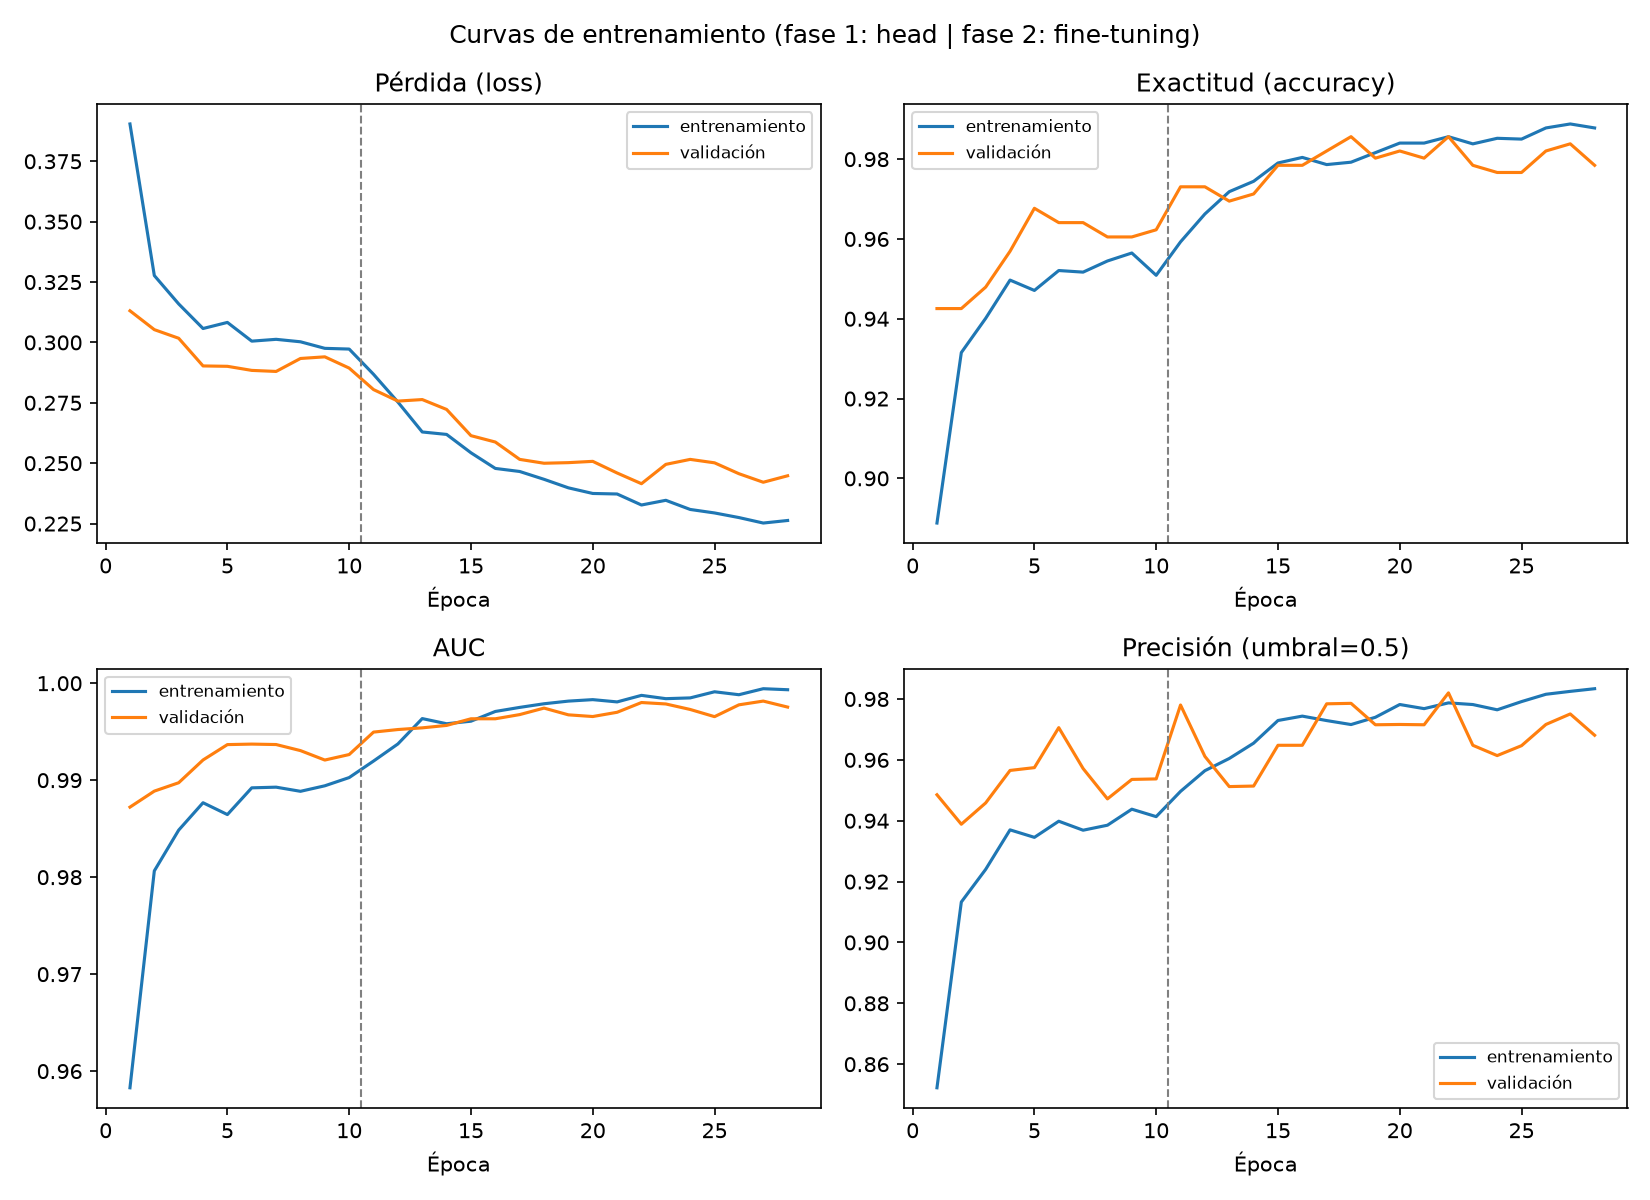
\includegraphics[width=0.92\textwidth]{images/C9/curvas_entrenamiento.png}
    \caption{Curvas de entrenamiento y validación para el clasificador de corteza (fases 1 y 2).}
    \label{fig:curvas_entrenamiento}
\end{figure}

Asimismo, la Figura~\ref{fig:metricas_balanceadas} ilustra la evolución de la exactitud balanceada y del puntaje $F_{0.7}$ en el conjunto de validación durante ambas fases, corroborando que el modelo mejoró de forma continua su capacidad de discriminación sin favorecer artificialmente a la clase mayoritaria.

\begin{figure}[H]
    \centering
    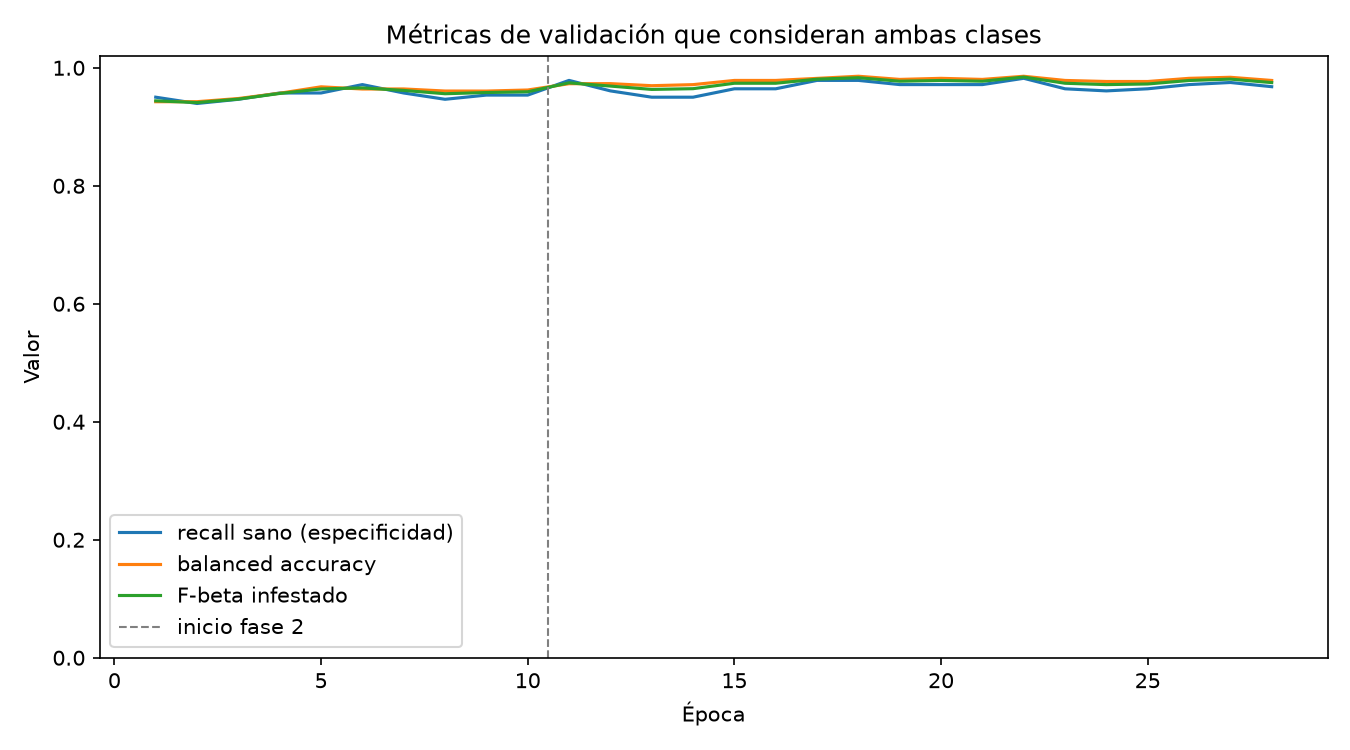
\includegraphics[width=0.85\textwidth]{images/C9/metricas_balanceadas.png}
    \caption{Evolución de la exactitud balanceada y la puntuación $F_\beta$ en validación.}
    \label{fig:metricas_balanceadas}
\end{figure}

\subsubsection{Optimización del umbral de decisión}
\label{subsubsec:umbral-optimo}

En aplicaciones de detección fitosanitaria, utilizar el umbral probabilístico por defecto de 0.5 suele ser subóptimo debido a las implicaciones asimétricas entre los errores de clasificación: clasificar erróneamente un árbol sano como infestado genera costos de inspección innecesarios, mientras que no detectar un árbol infectado permite la dispersión de la plaga.

Por esta razón, se realizó una búsqueda exhaustiva del umbral óptimo de decisión evaluando la métrica $F_{0.7}$ de forma estricta sobre el **conjunto de validación** (sin utilizar el conjunto de prueba para preservar la objetividad de los resultados finales). A partir de este procedimiento, se determinó como umbral óptimo:

\begin{equation}
    \tau_{\text{óptimo}} = 0.5791
\end{equation}

Con este umbral de corte, el modelo alcanzó en el conjunto de validación una precisión de 0.986, una exhaustividad (*recall*) de 0.986 y una puntuación $F_{0.7}$ de 0.986.

\subsubsection{Evaluación final en el conjunto de prueba independiente}
\label{subsubsec:evaluacion-test}

Una vez fijado el umbral óptimo $\tau = 0.5791$, se procedió a evaluar el modelo sobre el conjunto de prueba de 519 imágenes nunca antes vistas por la red. La Tabla~\ref{tab:metricas_test} presenta las métricas cuantitativas desglosadas por clase.

\begin{table}[H]
\centering
\small
\setlength{\tabcolsep}{5pt}
\caption{Métricas de evaluación final en el conjunto de prueba con umbral $\tau = 0.5791$.}
\label{tab:metricas_test}
\renewcommand{\arraystretch}{1.2}
\begin{tabular}{|l|c|c|c|c|}
\hline
\textbf{Clase} & \textbf{Precisión} & \textbf{Exhaustividad (\textit{Recall})} & \textbf{Puntaje $F_1$} & \textbf{Soporte} \\
\hline
Sano & 95.45\% & 97.30\% & 96.37\% & 259 \\
\hline
Infestado & 97.25\% & 95.38\% & 96.31\% & 260 \\
\hline
\textbf{Exactitud global (\textit{Accuracy})} & \multicolumn{3}{c|}{\textbf{96.34\%}} & 519 \\
\hline
Promedio macro (\textit{Macro Avg}) & 96.35\% & 96.34\% & 96.34\% & 519 \\
\hline
Promedio ponderado (\textit{Weighted Avg}) & 96.36\% & 96.34\% & 96.34\% & 519 \\
\hline
\end{tabular}
\end{table}

El modelo obtuvo una exactitud global del \textbf{96.34\%}, superando holgadamente los criterios mínimos requeridos para herramientas de apoyo en campo. La clase infestado alcanzó una precisión del \textbf{97.25\%}, lo que minimiza la generación de falsas alarmas para los brigadistas, junto con un *recall* del \textbf{95.38\%}, garantizando la detección efectiva de la mayoría de los árboles afectados.

La Figura~\ref{fig:evaluacion_test} muestra la matriz de confusión obtenida y la curva Precision-Recall correspondiente sobre el conjunto de prueba. De las 260 muestras reales de árboles infestados, 248 fueron clasificadas correctamente como positivas y únicamente 12 fueron clasificadas erróneamente como sanas. Asimismo, de los 259 árboles sanos, 252 fueron dictaminados correctamente, registrándose solo 7 falsos positivos.

\begin{figure}[H]
    \centering
    \begin{subfigure}[b]{0.48\linewidth}
        \centering
        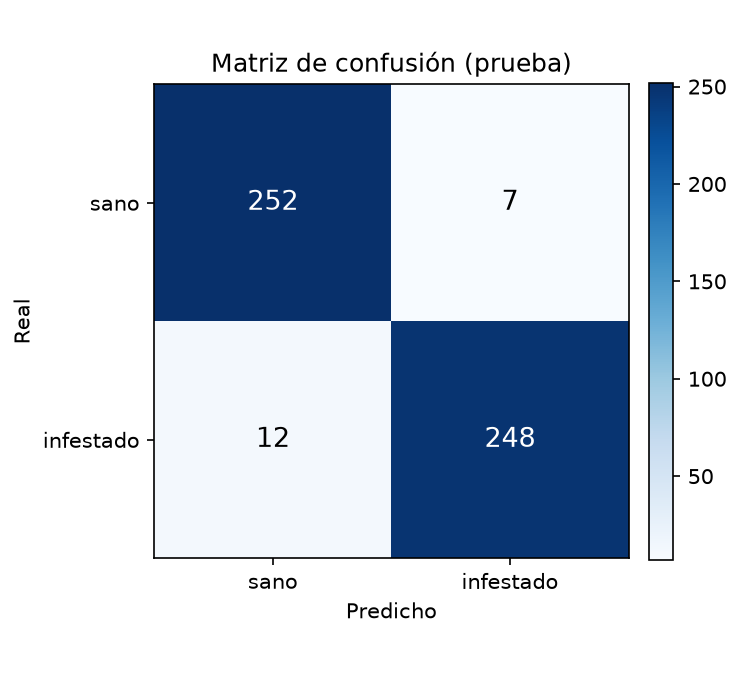
\includegraphics[width=0.98\linewidth]{images/C9/matriz_confusion_test.png}
        \caption{Matriz de confusión (Test).}
        \label{fig:matriz_confusion_test}
    \end{subfigure}
    \hfill
    \begin{subfigure}[b]{0.48\linewidth}
        \centering
        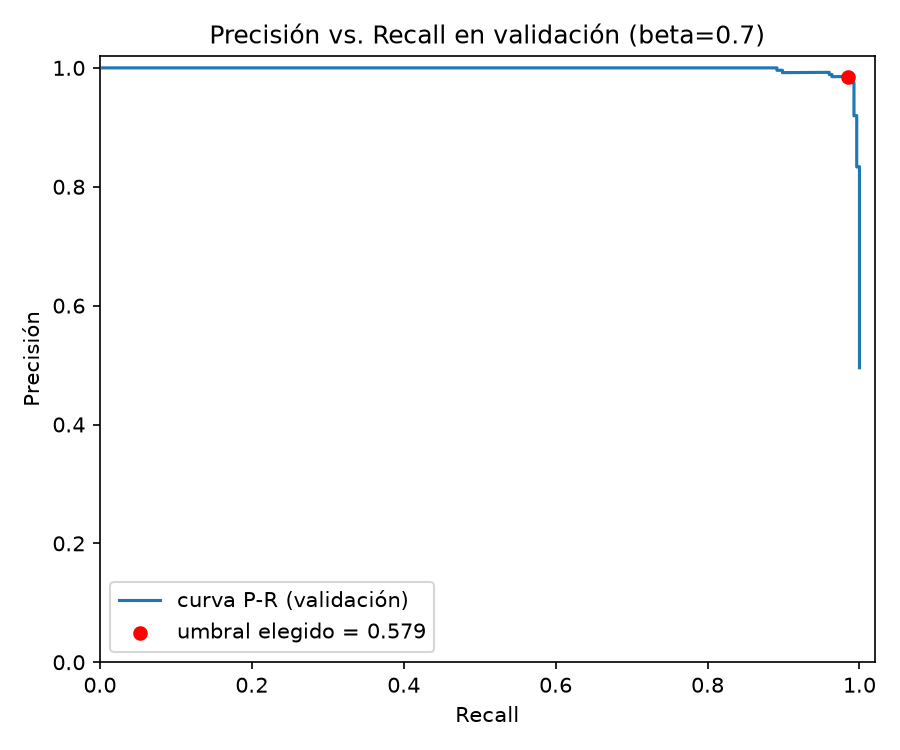
\includegraphics[width=0.98\linewidth]{images/C9/curva_precision_recall.png}
        \caption{Curva Precision-Recall.}
        \label{fig:curva_pr_test}
    \end{subfigure}
    \caption{Evaluación diagnóstica en el conjunto de prueba independiente.}
    \label{fig:evaluacion_test}
\end{figure}

Por otra parte, la Figura~\ref{fig:distribucion_probabilidades} presenta la distribución de probabilidades predichas para ambas clases, donde se evidencia una separación bimodal clara respecto a la frontera de decisión marcada por el umbral $\tau = 0.5791$.

\begin{figure}[H]
    \centering
    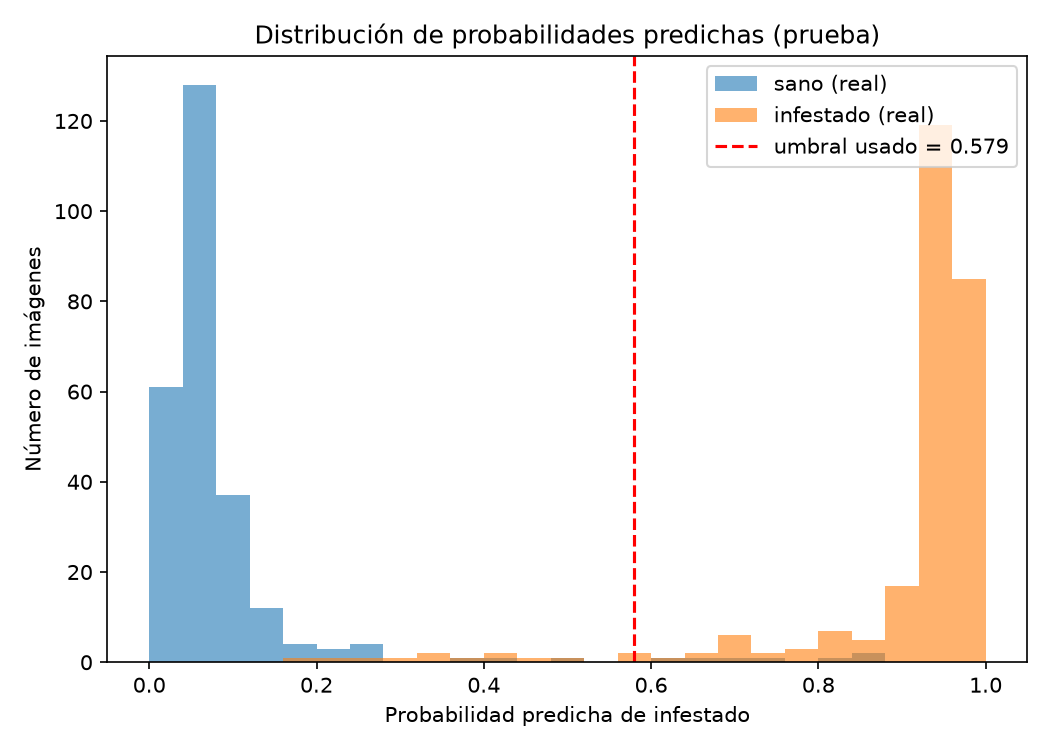
\includegraphics[width=0.85\textwidth]{images/C9/distribucion_probabilidades_test.png}
    \caption{Distribución de probabilidades predichas en el conjunto de prueba.}
    \label{fig:distribucion_probabilidades}
\end{figure}

\subsubsection{Exportación a TensorFlow Lite y verificación de paridad numérica}
\label{subsubsec:exportacion-tflite}

Con el fin de integrar el modelo entrenado dentro de la aplicación móvil de acuerdo con los requerimientos \textbf{RF-08} y \textbf{RF-09}, el modelo final de Keras fue convertido al formato embebido \textbf{TensorFlow Lite} (\texttt{bark\_classifier.tflite}), con un tamaño final en disco de \textbf{20.58~MB}, lo que cumple plenamente con la restricción de almacenamiento para dispositivos móviles.

Para verificar que el proceso de exportación y optimización no degradara la capacidad diagnóstica del clasificador, se ejecutó una prueba de paridad comparando las probabilidades predichas por el modelo original en Keras 3 frente al intérprete nativo de TensorFlow Lite sobre muestras del conjunto de prueba. La Tabla~\ref{tab:paridad_tflite} ilustra una muestra representativa de estas comparaciones.

\begin{table}[H]
\centering
\small
\setlength{\tabcolsep}{4.5pt}
\caption{Prueba de paridad diagnóstica entre el modelo Keras y el modelo TensorFlow Lite.}
\label{tab:paridad_tflite}
\renewcommand{\arraystretch}{1.2}
\begin{tabular}{|l|c|c|c|c|c|}
\hline
\textbf{Muestra evaluada} & \textbf{Keras (\%)} & \textbf{Clase Keras} & \textbf{TFLite (\%)} & \textbf{Clase TFLite} & \textbf{Diferencia (\%)} \\
\hline
\texttt{inf.webp} & 95.80\% & Infestado & 95.23\% & Infestado & 0.57\% \\
\hline
\texttt{alder\_2.jpg} & 7.68\% & Sano & 7.55\% & Sano & 0.13\% \\
\hline
\texttt{5549894.jpg} & 7.23\% & Sano & 8.58\% & Sano & 1.36\% \\
\hline
\texttt{alder\_1.jpg} & 6.35\% & Sano & 11.45\% & Sano & 5.10\% \\
\hline
\texttt{5543613.jpg} & 8.13\% & Sano & 7.41\% & Sano & 0.72\% \\
\hline
\texttt{5454221.jpg} & 7.41\% & Sano & 7.16\% & Sano & 0.25\% \\
\hline
\texttt{5500295.jpg} & 6.02\% & Sano & 6.21\% & Sano & 0.19\% \\
\hline
\texttt{5526018.jpg} & 3.69\% & Sano & 3.19\% & Sano & 0.50\% \\
\hline
\end{tabular}
\end{table}

Los resultados confirman que la asignación de clase es 100\% consistente entre ambos entornos, registrando diferencias porcentuales menores a nivel de probabilidad decimal atribuibles a la aritmética en punto flotante del runtime móvil, garantizando así una operación equivalente tanto en la nube como en el dispositivo de campo.
